% \chapter{Desenvolvimento/Implementação}\label{cap:development}

% Neste capítulo é descrito o trabalho de implementação, salientando os pontos mais relevantes da mesma, dificuldades  encontradas ou soluções técnicas inovadoras desenvolvidas ou aplicadas.  Em particular, se foi usado código desenvolvido por terceiros (por exemplo, código {\it open-source}), deve ser facilmente distinguível quais as funcionalidades originais do mesmo e o que foi necessário implementar para obter as funcionalidades desejadas.


\chapter{Arquitetura do sistema}\label{cap:development}
Neste capítulo, é abordado em detalhe a arquitetura e a estrutura adotada para a construção dos componentes do sistema. É importante compreender que o sistema foi concebido como um conjunto de módulos, com cada um desempenhando funções específicas, e quando operados em conjunto, esses módulos resultam na realização dos propósitos pensados para o sistema.

O sistema é estruturado fundamentalmente em camadas distintas, o backend, o frontend, e o banco de dados.

\begin{figure}[htbp]
	\centering
	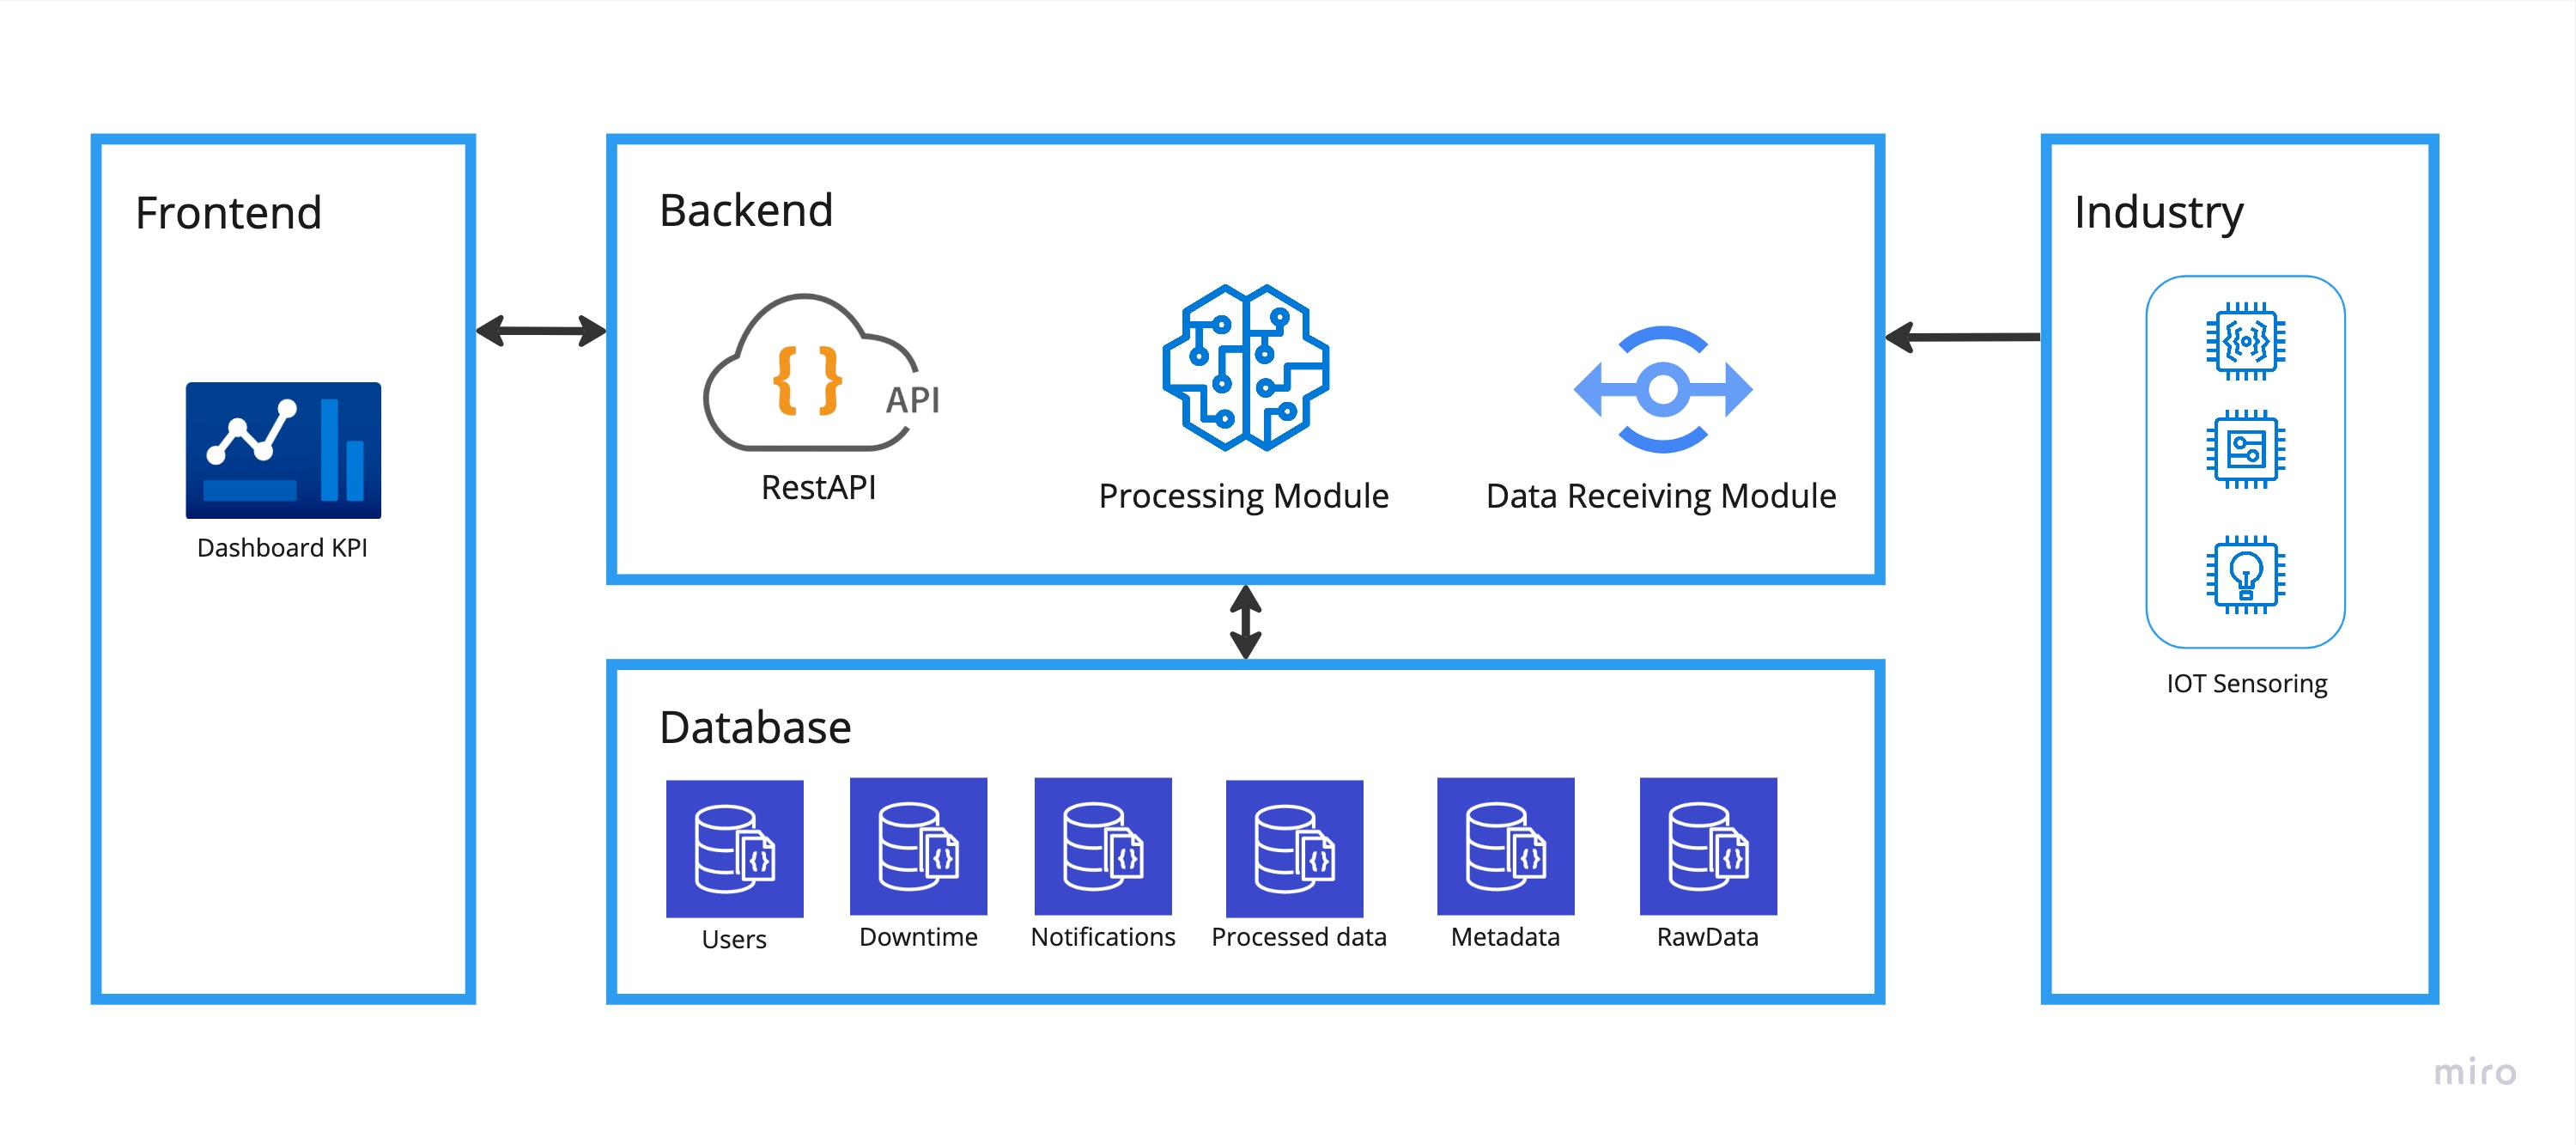
\includegraphics[width=\textwidth]{images/Architecture.jpg}
	\caption{System architecture.}
	\label{fig:systemAchitectureImage}
\end{figure}

%TODO Sigla api
O backend funciona como o núcleo do sistema. Sua principal função é a de receber os dados, processá-los conforme as regras estabelecidas nos requisitos e histórias de usuários e, armazená-los de maneira segura no banco de dados. Além das funções de armazenamento e processamento, ao backend também é atribuída a responsabilidade de disponibilizar esses dados por meio de uma interface de programação de aplicações (API), que pode ser acessada utilizando métodos HTTP. Esta API age como um intermediário entre a lógica central do sistema e as interfaces com as quais o usuário final interage, o frontend.

%TODO referencia para princípios de design e data visualization - Talvez referir a outra parte da dissertação que entra em mais detalhes
Por outro lado, o frontend é caracterizado como a interface visual que o usuário final acessa. Serve como meio pelo qual os usuários interagem com o sistema, enviando e recebendo informações. Esta camada é projetada para acessar, recuperar e apresentar os dados processados e armazenados pelo backend de uma maneira intuitiva e amigável, utilizando princípios de design e data visualization.

Como pode ser visto na figura ~\ref{fig:systemAchitectureImage}, na planta industrial, onde as máquinas com os sensores se encontram, os sensores enviam os dados para o sistema, que recebe eles por meio do modulo de recebimento de dados e os armazena no banco de dados. O modulo de processamento acessa os dados armazenados para realizar a agregação, e a API gerencia o acesso ao banco de dados, disponibilizando as informações para os usuários no frontend.

Nas seções seguintes, cada um desses componentes será explorado mais profundamente, passando por suas especificidades e interações.


\section[Arquitetura do backend]{Arquitetura backend}
%TODO Sigla HTTP
Nessa seção é abordado o funcionamento do backend. Ele está dividido em três partes, o modulo de recebimento dos dados dos sensores, o modulo de processamento onde é feita a agregação e analise estatística dos dados, e a API que gerencia o acesso as informações por meio de requisições HTTP.

Em relação a organização dos repositórios, a API e o modulo de recebimento de dados ficam no mesmo repositório, facilitando a comunicação entre eles. Já o modulo de processamento está em um repositório a parte, sendo a sua única função sendo ler o banco de dados, processar os dados, e armazenar os resultados.

\subsection{Modulo de Recebimento de dados}
Para o modulo de recebimento de dados, inicialmente, destaca-se a classe \texttt{SensorConnection}, cuja a função é gerenciar e manter a conexão com a rede de sensores. Essa classe faz a transmissão dos dados recebidos à uma função designada \texttt{save\_data\_func}, assegurando que os dados sejam encaminhados para manipulação apropriada.

Na próxima parte da arquitetura, é utilizada a classe \texttt{IotSensorConnection}, que se origina da interface \texttt{IotSensorConnectionInterface}. Esta interface foi criada para garantir a adaptabilidade do sistema, facilitando a integração de diferentes tipos de recebimentos de dados, como por exemplo, uma classe destinada a gerar dados dos sensores em um ambiente de desenvolvimento, onde não há acesso ao sensor real. A classe \texttt{IotSensorConnection}, quando instanciada, é encarregada de estabelecer a conexão, e criar uma nova thread que opera como um ouvinte ativo, monitorando a chegada de novas informações. Ao perceber a recepção de novos dados, a classe direciona estas informações para uma terceira entidade, a qual detém a responsabilidade de aplicar as regras de negócio.

Esta terceira entidade é a classe \texttt{SensorsRepository}, que quando acionada com dados oriundos dos sensores, tem a responsabilidade de avaliar a informação com base nos parâmetros estabelecidos, decidindo se é necessário acionar um alerta, e tornar os dados do sensor acessíveis via API, garantindo que esses dados estejam disponíveis para serem transmitidos em tempo real, via stream, para todos os usuários conectados. Além do mais, o dado é salvo no banco de dados, especificamente na coleção de dados brutos do data lake, \texttt{Raw Data}. Uma vez salvos no banco de dados, estes dados brutos estão disponíveis para serem processados pelo módulo de processamento.

A disponibilização dos dados pela classe \texttt{SensorsRepository} acontece por meio da instancia da classe \texttt{SensorValue}, que com o método \texttt{update\_current\_sensor\_value} atualiza os dados em memoria que são acessados pelos usuários conectados.

O diagrama que mostra a organização dessas classes pode ser visto na figura ~\ref{fig:receiveData}. Este design assegura que os dados brutos dos sensores sejam efetivamente recebidos, avaliados e armazenados.

No capítulo~\ref{cap:implementation}, é aprofundado nos detalhes de implementação desse módulo.


\begin{figure}[htbp]
	\centering
	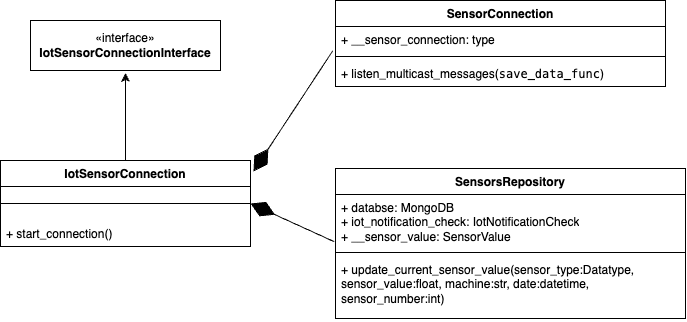
\includegraphics[width=\textwidth]{images/recebimento_dados.png}
	\caption{Module to receive sensor data.}
	\label{fig:receiveData}
\end{figure}


\subsection{Modulo de processamento de dados}\label{subsec:moduloProcessamento}
O módulo de processamento de dados foi desenvolvido para garantir que os dados brutos coletados sejam processados, fornecendo a análise estatística que é exibida para os usuários.

O código é executado quando é invocada uma função específica encarregada de realizar uma série de operações. Primeiramente, uma lista é constituída contendo as coleções do banco de dados responsáveis pelo armazenamento tanto dos dados brutos quanto dos dados já processados. Simultaneamente, uma segunda lista é gerada, representando as máquinas que enviaram informações para o sistema.

Com essas listas, inicia-se um procedimento iterativo, em que, para cada máquina identificada, os dados disponíveis são lidos, submetidos a um processo de análise estatística, após o qual os resultados obtidos são registrados na coleção de dados processados. Essa análise estatística adota o método do Box Plot.

%TODO Referencia para um artigo explicando sobre boxPlot
O Box Plot, também conhecido como diagrama de caixa, é uma ferramenta gráfica utilizada para representar a variação de dados observados de uma variável numérica por meio de quartis. Na figura ~\ref{fig:boxplot}, pode ser visto o retângulo formado pelo primeiro quartil (Q1), mediana e terceiro quartil (Q3), que fornecem uma noção sobre a centralidade e dispersão dos dados, enquanto as "antenas" estendem-se para mostrar a amplitude completa dos dados, ajudando assim na identificação de possíveis outliers.

Ao adotar o Box Plot, o sistema garante uma compreensão robusta da distribuição dos dados, identificando não apenas tendências centrais, mas também variações e potenciais anomalias.

\begin{figure}[htbp]
	\centering
	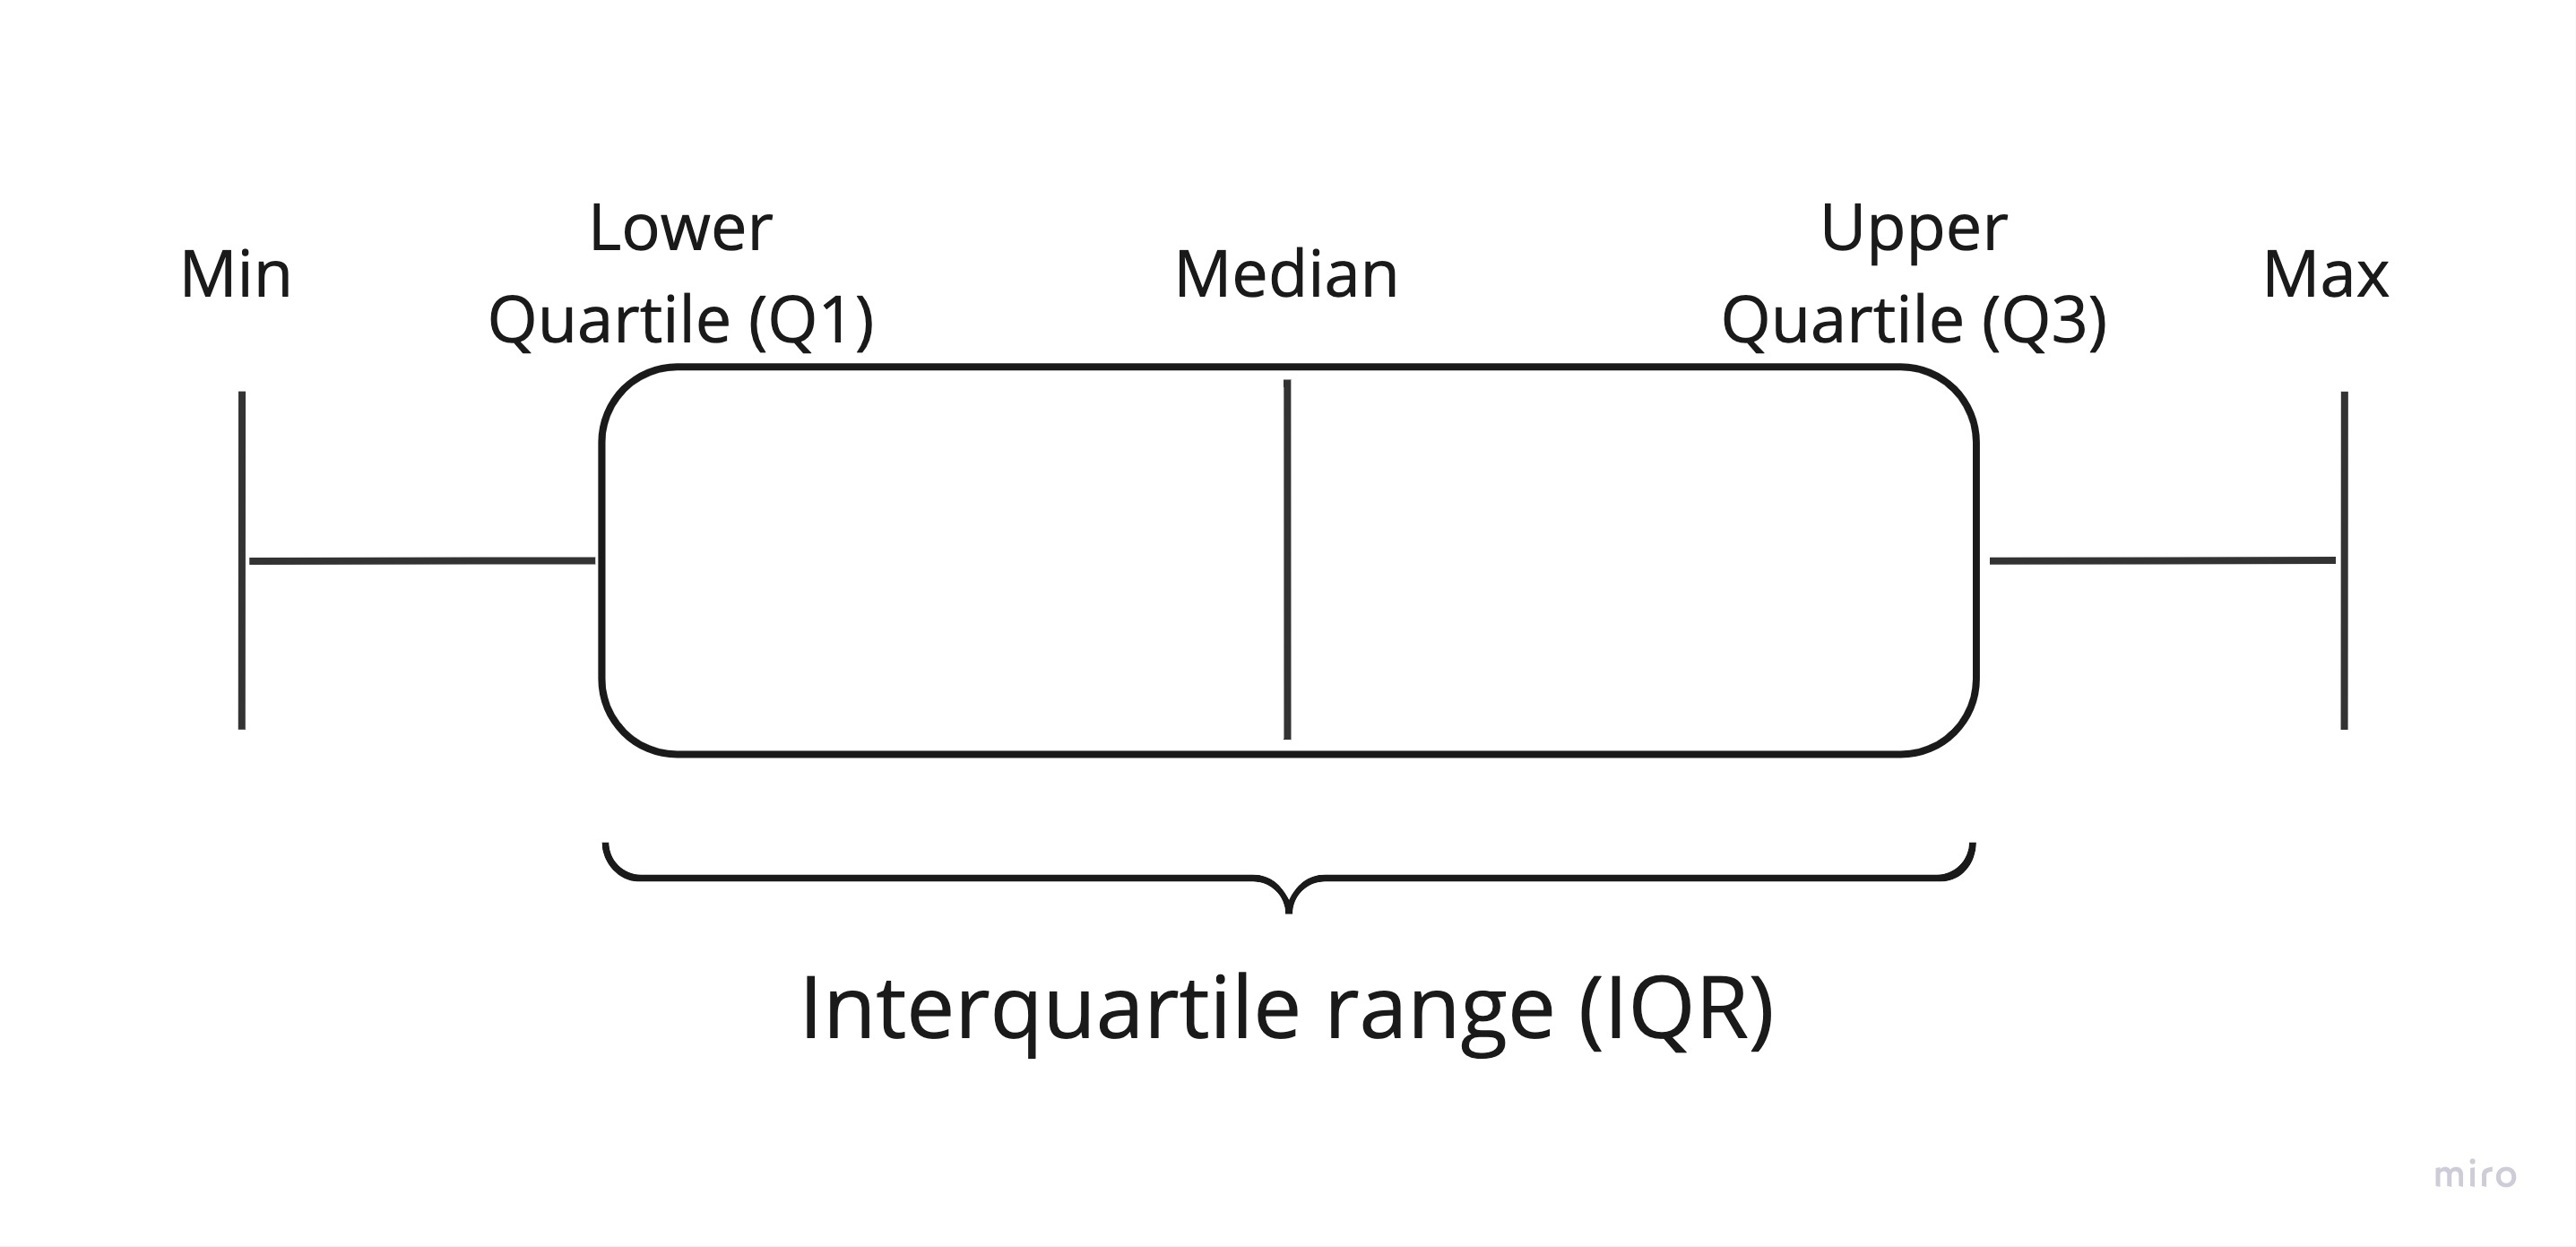
\includegraphics[width=\textwidth]{images/boxplot.jpg}
	\caption{BoxPlot.}
	\label{fig:boxplot}
\end{figure}


\subsection{API}\label{subsec:apiArchitecture}
A API foi estruturada em pequenos sub-módulos, cada um focado em um contexto específico. Esta modularização assegura que cada parte da API tenha uma única responsabilidade. Em cada módulo, há uma segmentação composta por: a camada de \textit{controller}, destinada a receber e gerenciar as requisições HTTP; a camada de serviço, que serve para processar a informação e aplicar as respectivas regras de negócio; e a camada de repositório, cujo papel é estabelecer uma ponte com o banco de dados, acessando e disponibilizando os dados necessários. A figura ~\ref{fig:api_organization} representa a organização de pastas que foi utilizada para essa arquitetura.

\begin{figure}[htbp]
	\centering
	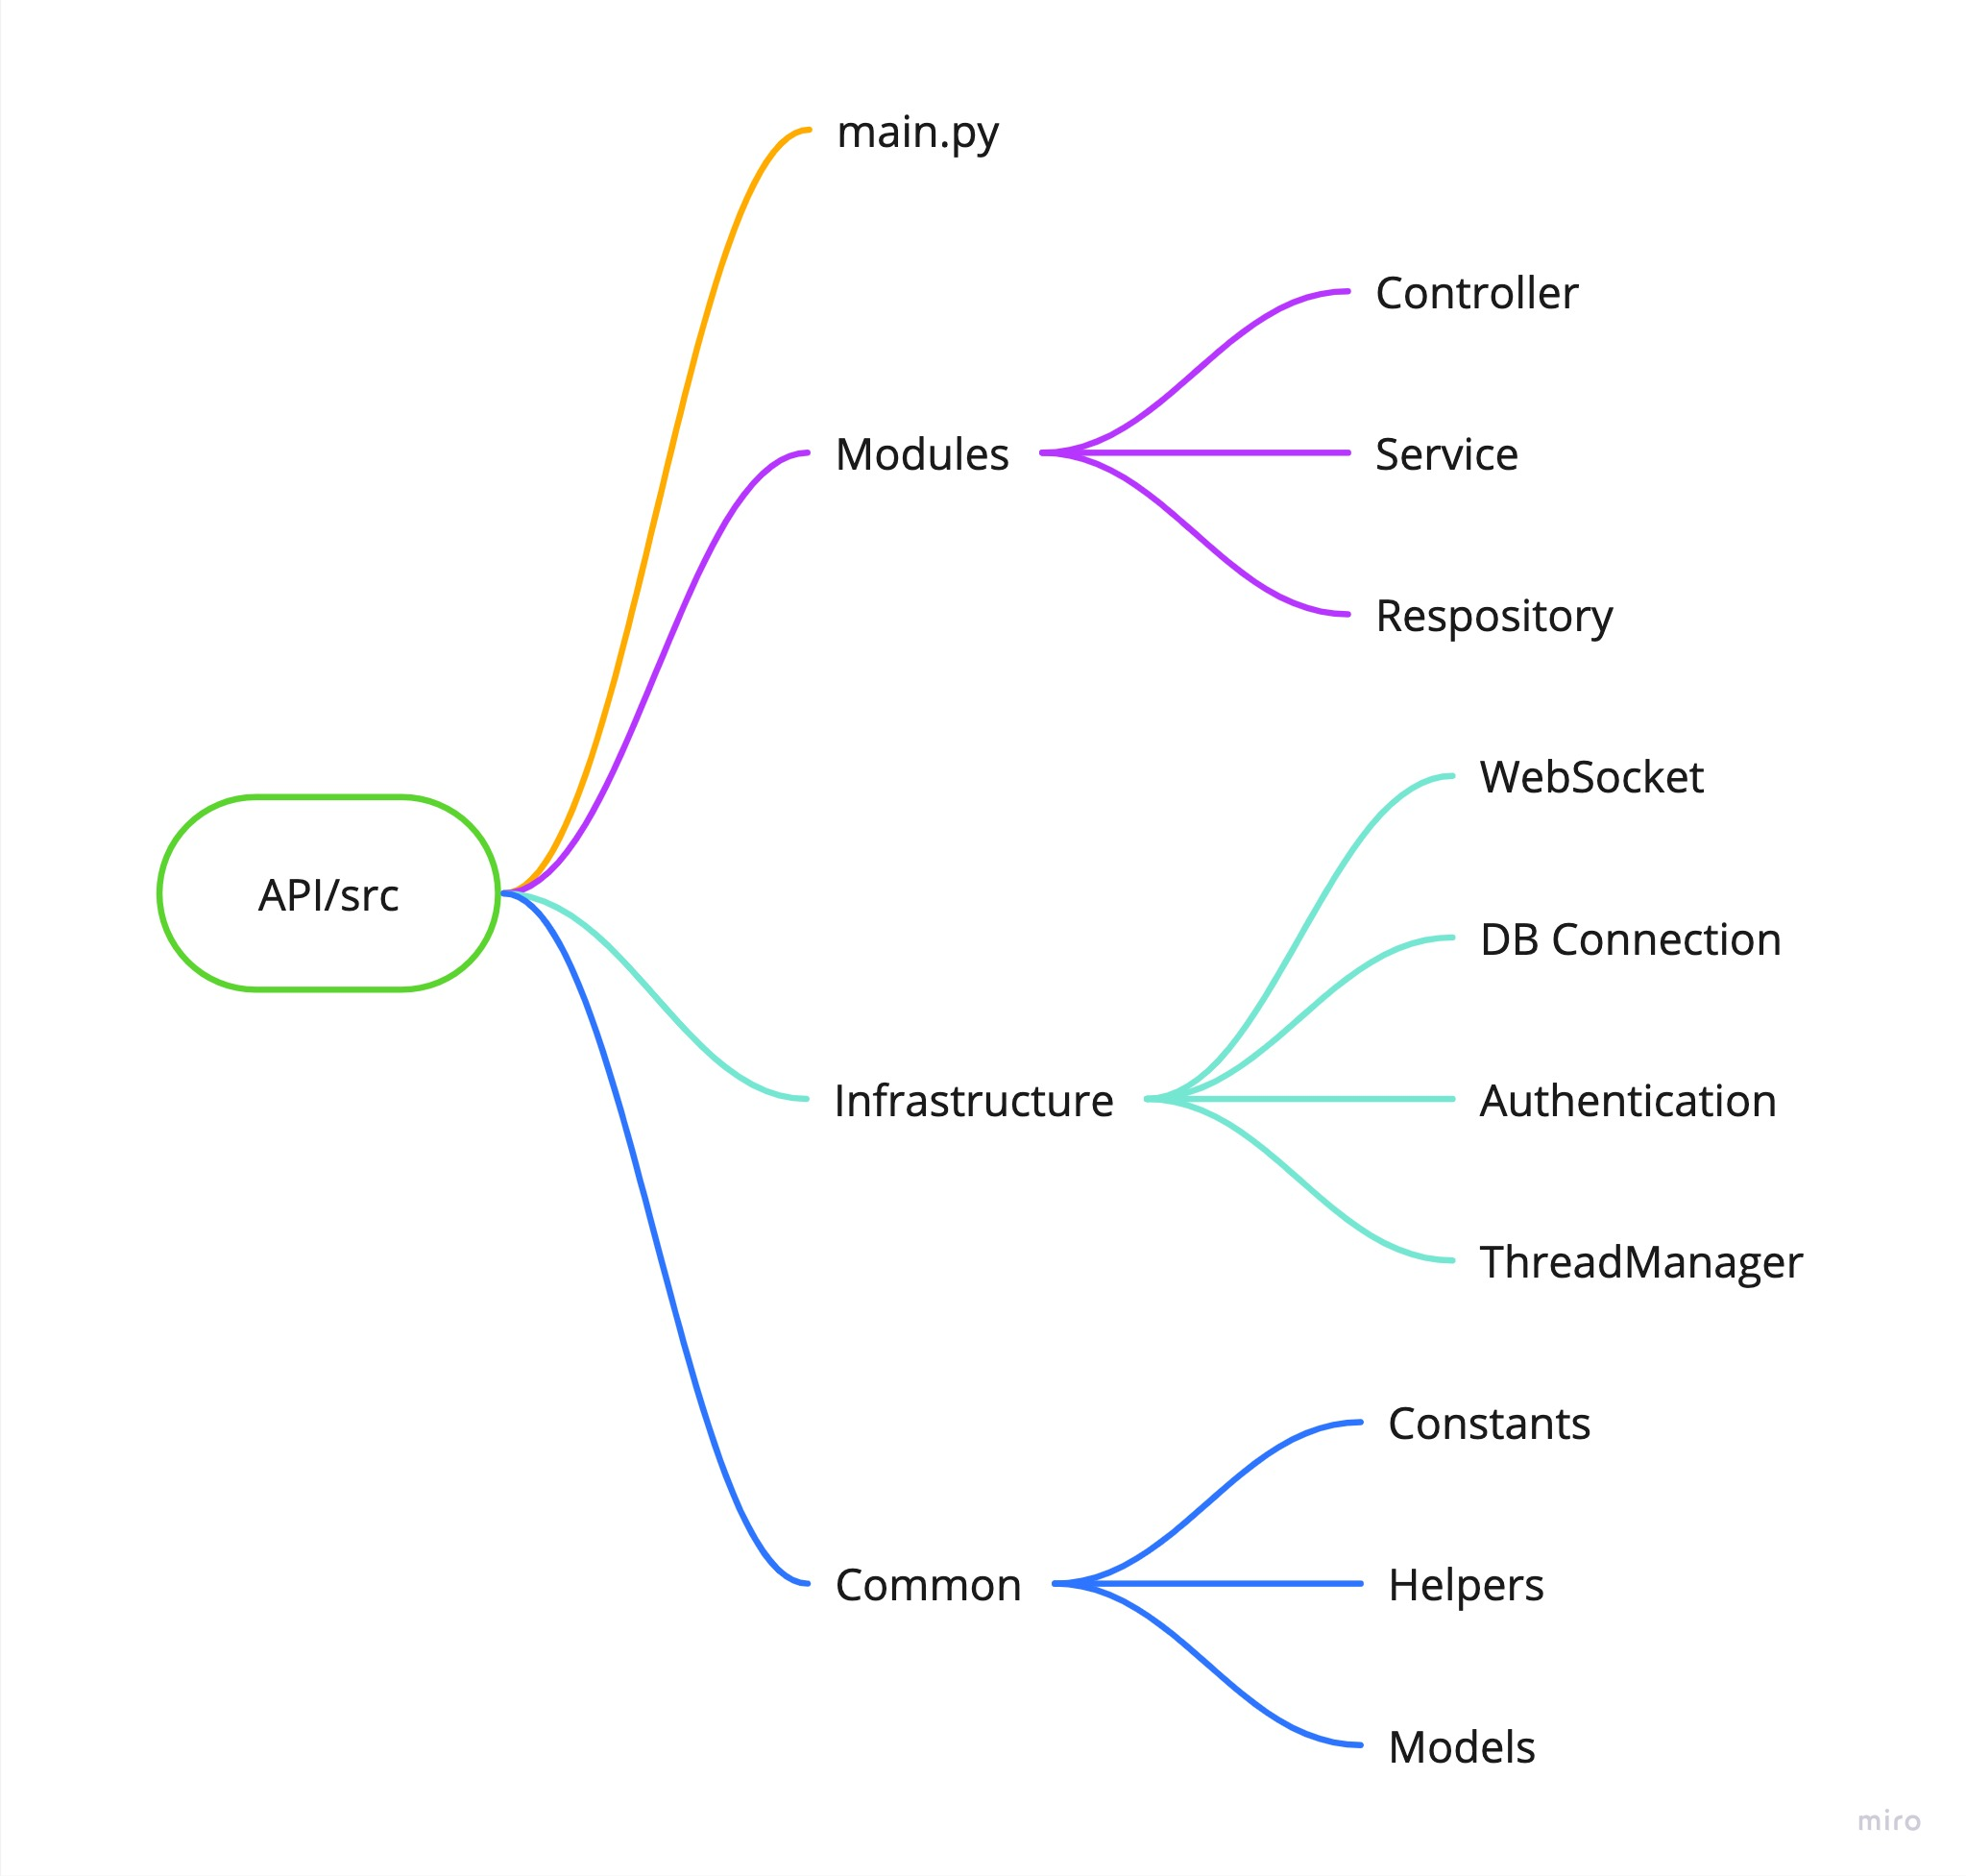
\includegraphics[width=\textwidth]{images/API_Organization.jpg}
	\caption{API Organization.}
	\label{fig:api_organization}
\end{figure}

Quando uma solicitação é enviada à API, a primeira interação acontece com a camada de \textit{controller}. Uma vez recebida, essa requisição é direcionada à camada de serviço, onde as regras de negócio são aplicadas. A camada de serviço se comunica estreitamente com a camada de repositório, que detém a responsabilidade de acessar o banco de dados e trazer informações precisas, adequadas às demandas do módulo em questão.

Os módulos implementados na API com a lógica descrita são:
\begin{itemize}
	\item \textbf{Downtime:} Responsável por gerenciar o acesso aos dados de paragem armazenados para teste no sistema.
	\item \textbf{IOT Sensors:} Responsável por gerenciar o acesso aos dados referentes aos sensores das maquinas na fabrica.
	\item \textbf{Notification:} Responsável por gerenciar o acesso as notificações geradas pelo sistema, e também as conexões web sockets para envio de notificações.
	\item \textbf{User:} Responsável por gerenciar o acesso aos dados dos usuários, assim como realizar as operações de login e logout. 
\end{itemize}

Além dessas camadas modulares, existe uma área especifica na API para o armazenamento de códigos comuns a todos os módulos. Esta seção engloba diversas funções úteis, modelos de classes, valores constantes e configurações padrão. Tais elementos garantem uma maior coesão e reduzem a repetição de código, otimizando o desempenho geral. Dentre as configurações padrão, merecem destaque o inicializador que estabelece o acesso ao banco de dados, middleware de autenticação, conexão web socket para envio de notificações, e o inicializador de novas \textit{threads}. Este último é utilizada para operações assíncronas que são executadas em paralelo a operação da API, como aquelas executadas pelo módulo de recebimento de dados.

\section[Arquitetura do frontend]{Arquitetura do frontend}
%TODO referencia para a doc do next
Utilizando o \textit{Next.js} como framework, o frontend segue uma estrutura básica já estabelecida pelo mesmo.

As rotas do sistema residem na pasta \texttt{pages}, alinhadas com as diretrizes do framework. Já os layouts que servem de base para cada página estão localizados na pasta \texttt{layouts}.

%TODO Referencia react
Os componentes \textit{React} são a fundação de cada página e layout e estão organizados em uma camada específica, permitindo que sejam reutilizados em várias partes da aplicação.

%TODO referencia para o typescript
Com a adoção do \textit{Typescript}, modelos definem os tipos de estrutura de dados utilizados. Estes são mantidos na pasta \texttt{types}, estabelecendo contratos de formato de dados para o frontend. Isso minimiza erros e potencializa a eficiência no desenvolvimento.

A \textit{Context API} do React é empregada para gerir dados nos componentes, permitindo o compartilhamento centralizado de informações, como pode ser visto na figura ~\ref{fig:FrontendOrganization}. Esta abordagem otimiza a maneira como os dados são acessados e distribuídos no sistema, otimizando a organização da arquitetura.

\begin{figure}[htbp]
	\centering
	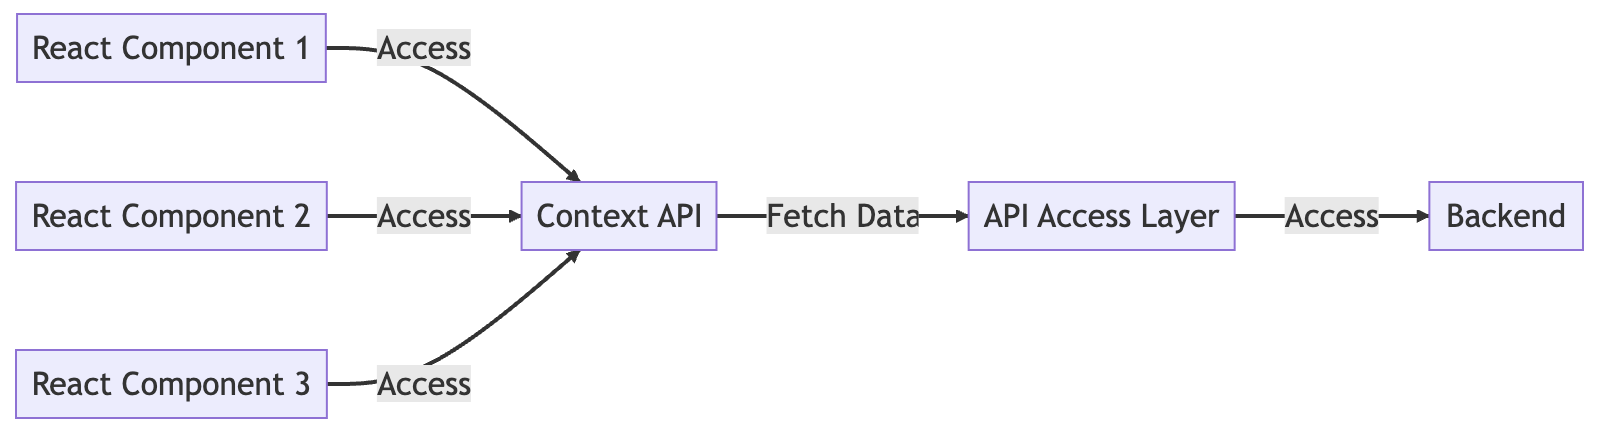
\includegraphics[width=\textwidth]{images/components_frontend.png}
	\caption{Frontend organization.}
	\label{fig:FrontendOrganization}
\end{figure}

Existe uma camada específica para acesso externo, que administra a comunicação com a API e as conexões \textit{WebSocket}. Esta é acessada apenas pelos contextos para atualização e recuperação de dados.

Por fim, há uma pasta dedicada para armazenar códigos recorrentes, contendo funções auxiliares, temas e \textit{assets}, facilitando o desenvolvimento e manutenção ao proporcionar uma estrutura clara e coesa.


\section{Containers}

%TODO Referencia para explicar sobre containers
Containers são tecnologias que permitem isolar aplicações em ambientes específicos com todas as suas dependências, bibliotecas e configurações necessárias, sem a sobrecarga de máquinas virtuais completas. Isso garante que a aplicação funcione de maneira idêntica em diferentes ambientes, desde o desenvolvimento até a produção. Na figura ~\ref{fig:container} é possível visualizar como é o funcionamento dos containers dentro do sistema operacional do  host.

\begin{figure}[htbp]
	\centering
	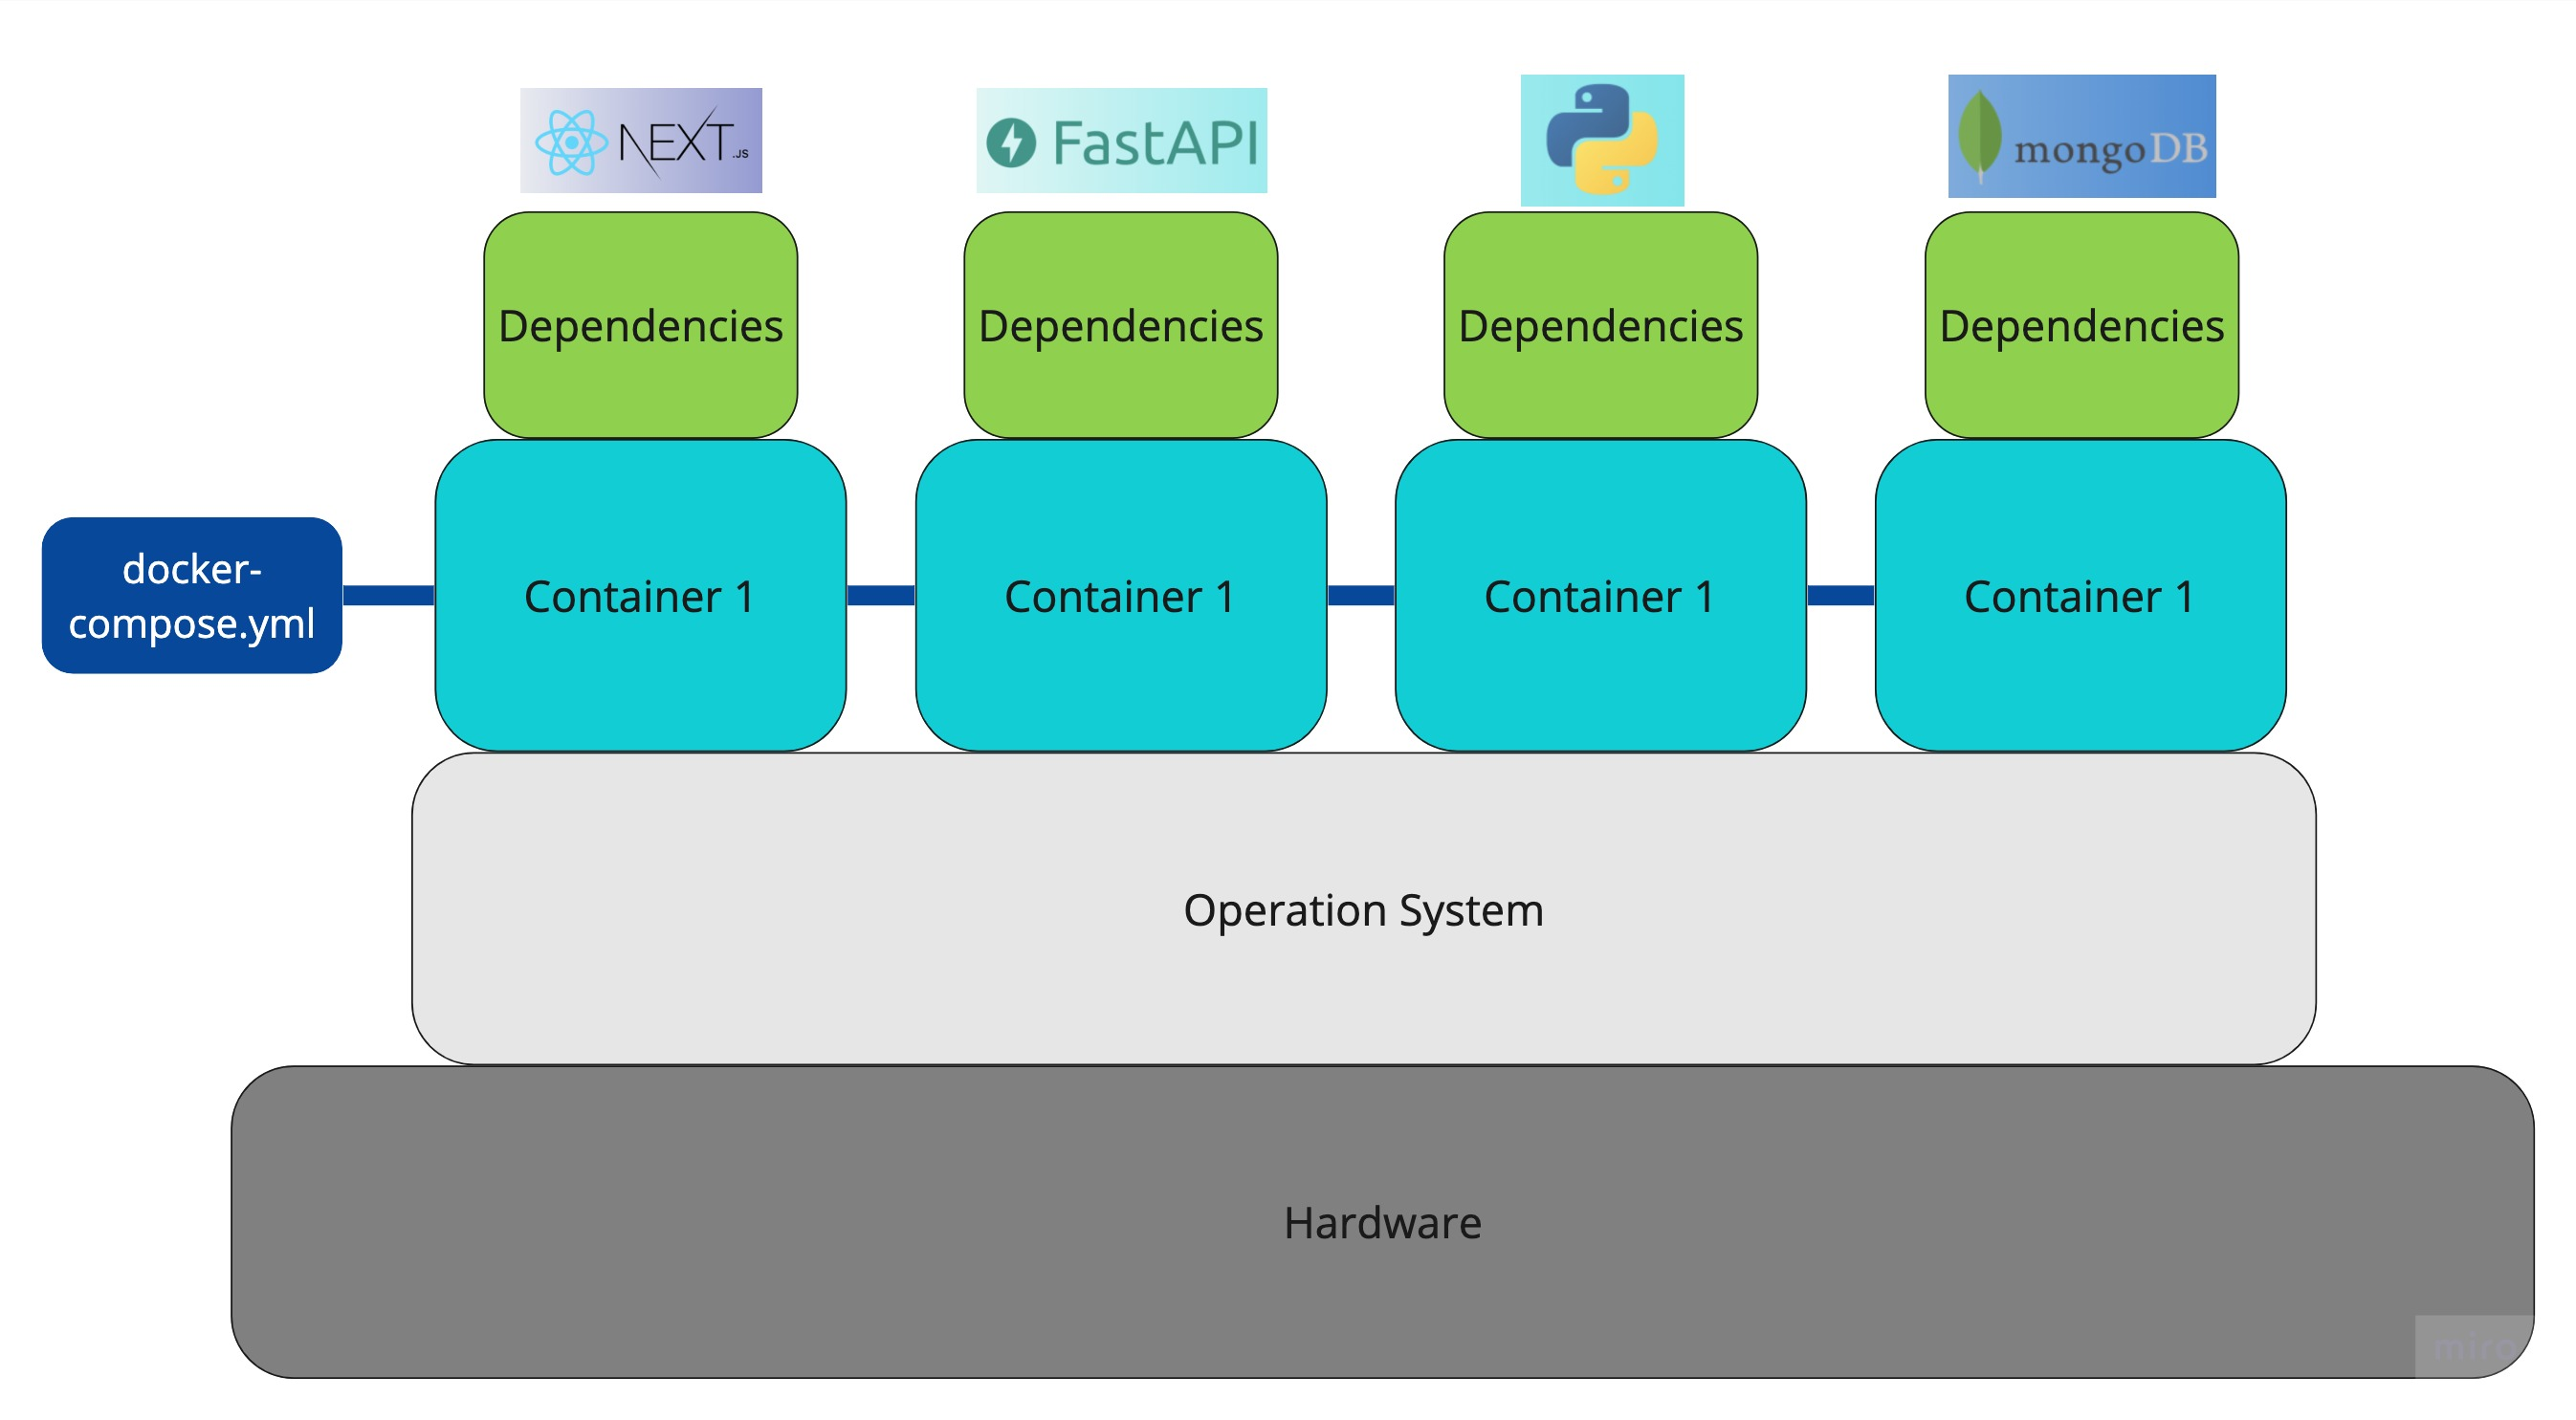
\includegraphics[width=\textwidth]{images/container.jpg}
	\caption{How container works.}
	\label{fig:container}
\end{figure}

%TODO Referencia para o docker
Dentro do universo dos containers, o \textit{Docker} foi a ferramenta selecionada para este projeto. Diversos fatores influenciaram essa decisão, incluindo uma documentação abrangente, uma comunidade ativa e a presença de uma ampla variedade de conteúdos disponíveis. Além disso, o Docker simplifica a definição, criação e execução de containers, tornando-se uma solução robusta para a implantação de aplicações.

O sistema adota alguns containers para organizar e gerenciar as várias partes da aplicação:
\begin{itemize}
    \item \textbf{Frontend}: Um container dedicado ao frontend, construído com \textit{NextJs}.
    \item \textbf{Backend}: Dividido em dois containers distintos:
	\subitem Um que abrange a API e o módulo de recebimento de dados;
	\subitem E outro que é voltado especificamente para o módulo de processamento de dados;
    \item \textbf{Banco de Dados}: Um container para o banco de dados MongoDB, garantindo isolamento e eficiência na gestão dos dados.
\end{itemize}

%TODO Referencia para redes do docker
A comunicação entre os containers é viabilizada através de uma rede \textit{bridge} providenciada pelo Docker. Esta rede é uma interface de software criada no host que permite que containers comuniquem entre si e com o host, assegurando a conectividade necessária entre os diferentes módulos da aplicação. Com isso é adicionada uma camada a mais de segurança na aplicação, já que toda conexão externa deve ser feita por meio dessa rede. A conexão com rede externa é feita por meio de um web sever, explicado na seção ~\ref{sec:webserver}.

%TODO referencia para volume
Para garantir a persistência dos dados e evitar a perda de informações vitais, foi empregado o conceito de \textit{volumes} do Docker na arquitetura do sistema. Volumes são espaços designados no sistema host que podem ser acessados e utilizados pelos containers. No contexto deste projeto, um volume foi especificamente configurado para o banco de dados MongoDB. Assim, mesmo que o container do banco de dados seja reiniciado ou removido, a base de dados se mantém intacta e disponível, devido à sua armazenagem no volume, que opera independentemente do ciclo de vida do container.

%TODO referencia para o docker compose
%TODO referencia para o arquivo YAML
Com a necessidade de gerenciar múltiplos containers, configurações de rede e volumes de forma coesa e simplificada, foi adotado o \textit{Docker Compose} na arquitetura do sistema. O Docker Compose permite a definição e execução de aplicações multi-container usando um arquivo YAML. Esse arquivo contém todas as configurações necessárias para inicializar e interconectar os containers. Assim, ao invés de executar uma série de comandos para iniciar cada container individualmente, é possível, através do Docker Compose, iniciar todo o sistema com um único comando. Essa abordagem não apenas simplifica o processo de deploy e desenvolvimento, mas também garante que as configurações de rede e volume sejam consistentemente aplicadas em cada execução.

%TODO Referencia para os benefícios do docker
A utilização de containers no projeto trouxe vantagens. Primeiramente, garantiu a consistência entre os ambientes de desenvolvimento e produção. Adicionalmente, a modularização proporcionada pelos containers facilita a escalabilidade e manutenção do sistema, permitindo atualizações e alterações de forma ágil e segura a medida que o sistema for crescendo. Por último, a utilização de containers facilita a portabilidade do sistema, podendo ser executado em diversos tipos de servidores e sistemas, bastando ter a instalação do docker.


\section{Web Server}\label{sec:webserver}

%TODO referencia para o NGINX
%TODO Sigla NGINX
Dentro da arquitetura proposta, com containers executando diferentes partes da aplicação, foi utilizado o \textit{NGINX} para ser o intermediário no tráfego de requisições, assegurando a distribuição correta das solicitações para cada container. 

O método empregado para tal é o de proxy reverso. Em termos simples, o proxy reverso atua como uma interface entre o cliente e vários servidores, direcionando as solicitações dos clientes ao servidor adequado  (no contexto desse projeto, os containers), e assim, otimizando o uso dos recursos e garantindo uma resposta mais rápida e eficiente.

No que se refere a requisições específicas, aquelas que envolvem retorno em formato de stream ou estabelecem uma conexão \textit{WebSocket}, as configurações específicas foram feitas na configuração do \textit{NGINX}, sendo essas detalhadas no capítulo~\ref{cap:implementation},  dedicado à implementação. Ao receber uma requisição, o servidor \textit{NGINX} identifica, com base nela, qual container é o responsável pelo atendimento. Após essa identificação, são aplicadas as configurações adequadas, e a requisição é direcionada ao container correspondente para obter a resposta. Esse workflow pode ser visto na figura ~\ref{fig:nginx_workflow}.

\begin{figure}[htbp]
	\centering
	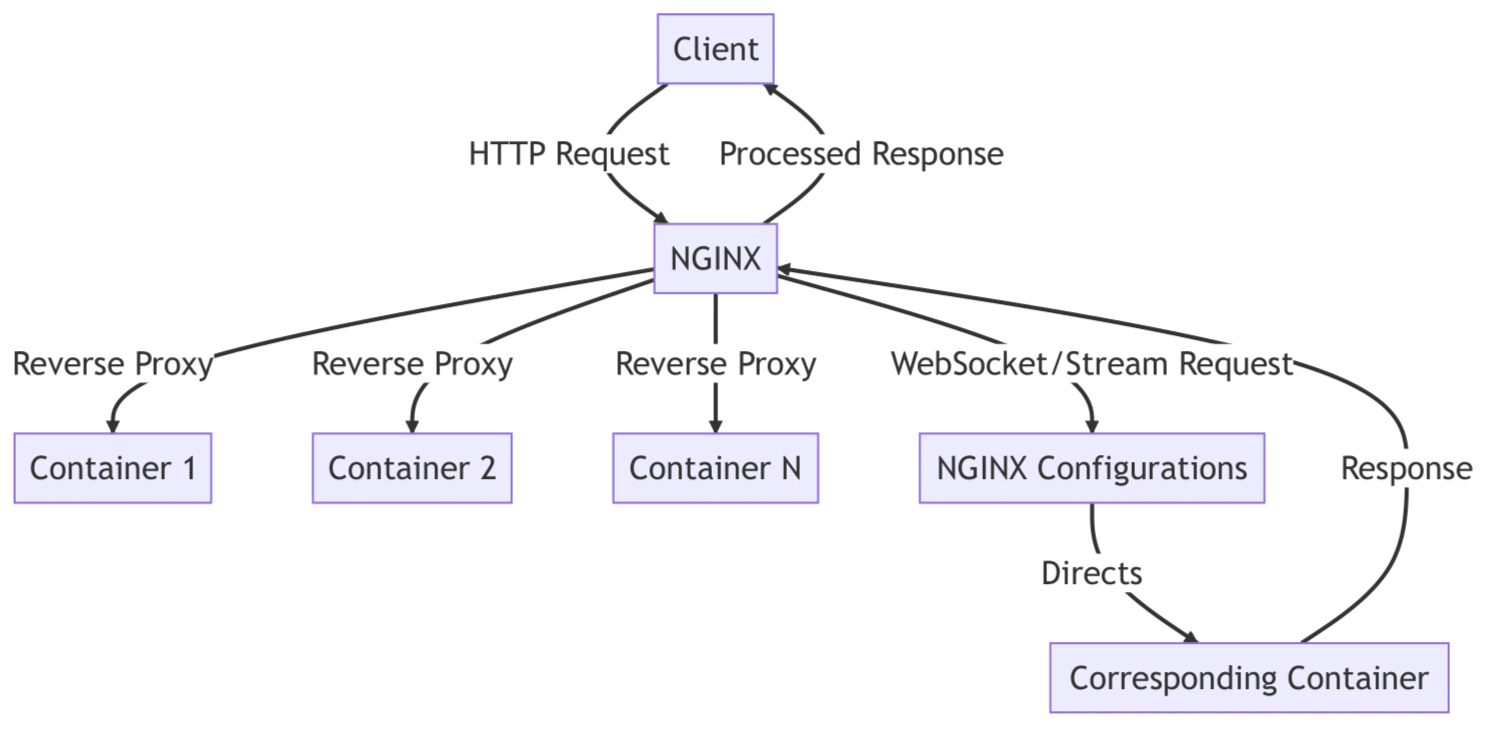
\includegraphics[width=\textwidth]{images/diagrama_nginx.png}
	\caption{NGINX workflow.}
	\label{fig:nginx_workflow}
\end{figure}

A incorporação do \textit{NGINX} trouxe alguns benefícios ao projeto. Um deles é a camada adicional de segurança: o \textit{NGINX} limita o acesso direto aos containers, servindo como uma barreira contra tentativas de acesso não autorizado. Adicionalmente, com o NGINX, o processo de escalabilidade torna-se mais simples e eficiente, graças à capacidade inerente do servidor em atuar como um balanceador de carga. Este balanceador de carga distribui o tráfego de entrada entre vários servidores, assegurando que nenhum servidor fique sobrecarregado. Esta funcionalidade não só melhora a performance geral como também proporciona uma maior disponibilidade do sistema, já que, em caso de falha de um servidor, o tráfego pode ser direcionado a outro que esteja operacional.
